%\documentclass[JIP,draft]{ipsj}
%\documentclass[JIP]{ipsj}

\documentclass[JIP]{apris}

\usepackage[dvips]{graphicx}
\usepackage{latexsym}

\def\Underline{\setbox0\hbox\bgroup\let\\\endUnderline}
\def\endUnderline{\vphantom{y}\egroup\smash{\underline{\box0}}\\}
\def\|{\verb|}

\setcounter{volume}{20}% vol20=2012
\setcounter{number}{4}% 1, 2, 3, 4
\setcounter{page}{1}

\received{2011}{7}{1}
%\rereceived{2011}{10}{1}   % optional
%\rerereceived{2011}{10}{31} % optional
\accepted{2011}{11}{5}

\usepackage[varg]{txfonts}%%!!
\makeatletter%
\input{ot1txtt.fd}
\makeatother%

\begin{document}

\title{code2vec for C: The Acquisition Method of Distributed Representation of the C Language with The TF-IDF Method}

\affiliate{IPSJ}{Faculty of Information Science and Electrical Engineering, Kyushu University}
\affiliate{JU}{Graduate School of Information Science and Electrical Engineering, Kyushu University}
\affiliate{F}{Fujitsu Kyushu Network Technologies Limited}

\author{Kotori Hieda}{JU}[hieda@f.ait.kyushu-u.ac.jp]
\author{Kenji Hisazumi}{IPSJ}[nel@slrc.kyushu-u.ac.jp]
\author{Hirofumi Yagawa}{F}
\author{Akira Fukuda}{IPSJ}[fukuda@f.ait.kyushu-u.ac.jp]


\begin{abstract}
Code2vec is a method for obtaining a distributed representation of program code. It obtains the embedding vector of program code through machine learning and predicts the label such as ‘method body’ representing the functionality of the code snippets. Thus, it is possible to obtain a distributed representation of the code snippet whose meaning is taken into account. In embedded system development, the non-object-oriented programming language C is often used, however code2vec is intended for object-oriented programming languages such as Java and C\#. Therefore, to apply code2vec to the C language, there are some problems that must be solved: labelling is difficult since the function name differs from that of the object-oriented language, and we need to develop a method of feature amount extraction from C language. In the following paper, we propose a method for extracting feature values from the C language programs and making use of the TF-IDF method for decomposing a given function name into both module-specific names and general operation names, as found in object-oriented languages.
% Code2vec is a method for obtaining a distributed representation of the program code. It obtains the embedding vector of program code through machine learning and predicts the label such as ``method body'' representing the functionality of the code snippets. Thus, it is possible to obtain a distributed representation of the code snippet whose meaning is taken into account. In the embedded system development, you often use the C language which is non-object-oriented, but code2vec is intended for object-oriented programming languages ​​such as Java and C\#. Therefore, to apply the code2vec to the C language,  there are some challenges that labeling is difficult since the naming of the function name is different from that of the object-oriented language and we need to consider a method of feature amount extraction from C language. In this study to apply code2vec to the C language programs, we propose a method for extracting feature value from the C language programs and TF-IDF method for decomposing a function name in a module-specific name and general operation name like the object-oriented language.
\end{abstract}

\begin{keyword}
code2vec, TF-IDF, C language, code snippet, function name estimation
\end{keyword}

\maketitle

%1
\section{Introduction}
In natural language processing, methods for obtaining distributed representations that take into account their meanings such as word2vec\cite{rong2014word2vec} have been proposed and applied in various ways. Current software development is supported in various ways using similar methods in program code, however there is room for improvement in both methods and applications. 
% In natural language processing, methods for obtaining distributed representations that take into account their meanings such as word2vec\cite{rong2014word2vec} have been proposed and applied in various ways.
% Software development is supported in various aspects using similar methods in program code, however there is room for improvement in both methods and applications.

Code2vec\cite{alon2019code2vec} has been proposed as a method for obtaining the distributed representation of a given program’s code. In this approach, it is possible to numerically express the code snippets and the relationship between them as real vectors. The main application of the distributed representations obtained by code2vec is to estimate the method name from the method body. Code2vec is designed for object-oriented languages such as Java and C\#. 
% Code2vec\cite{alon2019code2vec} has been proposed as a method for obtaining the distributed representation of the program code. In this approach, you can numerically express the code snippets and the relationship between them as real vectors. The main task to use distributed representations obtained by code2vec is such as estimation of the method name from the method body. Code2vec is for object-oriented languages such as Java and C\#.

C language is often used in embedded systems, however, as it is not an object-oriented language, it is not possible to directly apply C language to code2vec. In particular, when estimating the function name, estimation accuracy decreases because the function name itself contains both the module-specific name and general operation name.
% C language often used in embedded systems, however, is not an object-oriented language so you can not directly apply C language to code2vec. Especially in the task of estimating the function name, the estimation accuracy of the function name decreases because it contains both the module-specific name and general operation name.

In this study, we apply TF-IDF (Term Frequency Inverse Document Frequency)\cite{ramos2003using} to the function name to remove module-specific names based on the TF-IDF value. The TF-IDF value increases when a certain word appears frequently in a specific document, whilst only appearing infrequently in other documents. Since the module-specific name is unique within a document, its TF-IDF value is high. Therefore, we set a threshold for the TF-IDF value and delete the one with the highest value to leave only the operation name. By learning only operation names as function names, we aim to improve the accuracy of function name estimation. 
% In this study, we apply TF-IDF (Term Frequency Inverse Document Frequency)\cite{ramos2003using} to the function name to remove module-specific names based on the TF-IDF value. The TF-IDF value becomes higher when the word appears frequently in a given document, but the word hardly appears in multiple documents. Since the module-specific name is unique within a document, its TF-IDF value is high. Therefore, we set a threshold for the TF-IDF value and delete the one with high value to leave only the operation name. By learning only operation names as function names, we aim to improve the accuracy of function name estimation.

%2
\section{Analytical method}
In this section describing the analysis procedure of C language program code.

Since the C language program is made up of a plurality of files, it performs the processing for each file. First extracts a function definition. Function definition function name, arguments, return value, and a function body.

Since the function name is usually a compound word, to extract only the future general terms. To represent the delimiter of a word, the first letter of the word to upper case, and camel case to be in lower case otherwise, since the underscore is used, it extracts words in their separated. Further, the number is as a general term fried multi is inappropriate, to remove a number. do this, to subject the file of all of the C language programming code that is prepared.

 All occurrences number of documents about the word (DF) is calculated, and the entire dictionary. Also, to create a dictionary of frequency of appearance of each word (TF) for each file. Based on these dictionaries calculating the TF-IDF. TF-IDF word X in document A is word X in (document A frequency) / (the total sum of the frequency of occurrence of words) * log (total number of documents in the document a) / (calculated by the number of documents) that contain the word X. after calculating all the words of TF-IDF appearing in , to create a function name that you remove the following words threshold.

 Then analyzed following the implementation for other languages ​​.code2vec for extracting a feature value from the function body. Convert the function body parsing to the abstract syntax tree, extracts all terminal symbols in the tree. The extracted extracting a sequence of non-terminal symbols and terminal symbols connecting the terminal symbol to be. set to create all the combinations of terminal symbol as the path. This is a feature quantity.

 This, and a function name composed of general preferences and features extracted from the function body, learning using Code2vec.

%3
\section{Related research}
Cmu-seiの研究では、我々と似たような手法でC言語へのcode2vecの適用を試みていた。彼らはCとJavaのパーサーの違いや、Cにある関数宣言がJavaにはないことなどに着目し、我々と同様にClangとLLVMを使用し、関数を抽象化することで、code2vecのC言語への適用を試みていた。

Cmu-seiの研究では、我々と似たような手法でC言語へのcode2vecの適用を試みていた。彼らはCとJavaのパーサーの違いや、Cにある関数宣言がJavaにはないことなどに着目し、我々と同様にClangとLLVMを使用し、関数を抽象化することで、code2vecのC言語への適用を試みていた。
% code2vec has been proposed as a method for obtaining a distributed representation of the program code. In the conventional method, learning an identifier, such as appearing in the program code, it had gained a distributed representation. However identifier in the code it is often function code is different yet substantially similar. For example, in the operation for the sequence, and code for determining whether the specified element is present in the sequence, when there is specified elements in the array is a code that returns a value, the return is substantially the same structure value is different only. Accordingly, to reflect the distributed representation differences these delicate in Code2vec, After the code into an abstract syntax tree, the feature amount extracting a column of non-terminal symbols and terminal symbols connecting the two terminal symbols in the tree as the path to. This by learning based on the feature amount, it becomes possible to discern what structure also changes a slight difference by a function similar.


%4
\section{Conclusion}
表~?はcmu-seiと我々の関数名推定の結果の比較である。今回我々はGitHubのC言語のレポジトリのうちトップの50レポジトリを学習データとして比較している。これによると〜ということがわかった。
%  The code2vec In this research to apply the C language, illustrated the implementation of extracting a feature quantity using LLVM and Clang\cite{lattner2007clang}. In the task of estimating the function name from the function body, an identifier such as C language function name, since it is often composed of compound words and module specific name and general operation name, the time of learning we discussed that there is likely to be an obstacle. Furthermore, in order to solve this problem, we proposed a method of classifying the module-specific names and operation names using the function name of the C language TF-IDF. The results show that it is possible to extract only general operation name from the function name in the C language.

 The future challenges. Evaluation by applying the proposed method, such as evaluation by application to other identifier of the variable name, and the like not only the function name, and the like.

% \begin{table}[t]
%  \centering
%  \caption{TF-IDF手法を用いた推定結果}
%  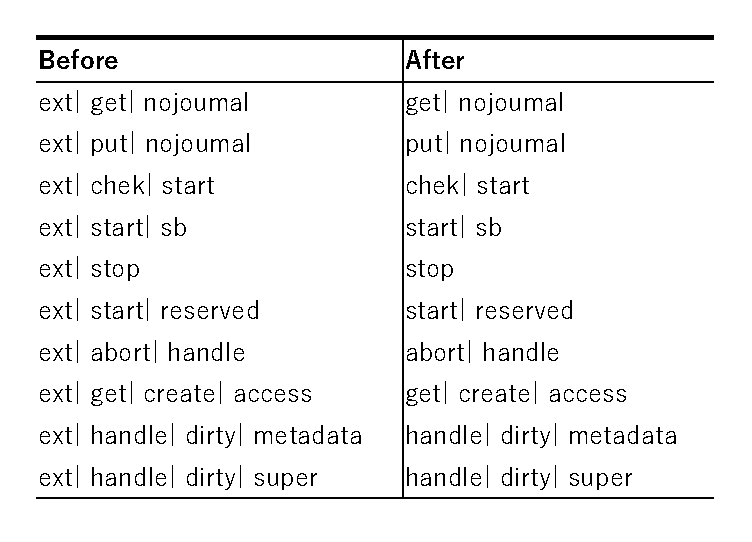
\includegraphics[width=1.0\hsize]{image/TF-IDF.eps} 
%  \label{table2} 
% \end{table}


\bibliographystyle{ipsjunsrt}
\bibliography{ebibsample}

% \begin{thebibliography}{99}
% \bibitem{companion}%1
% Goossens, M., Mittelbach, F., and Samarin, A.:
% {\it The LaTeX Companion},
% Addison Wesley, Reading, 
% Massachusetts (1993).

% \bibitem{latex}%2
% Lamport, L.: 
% {\it A Document Preparation System {\LaTeX} User's Guide \&
% Reference Manual}, 
% Addison Wesley, Reading, Massachusetts (1986).
% \end{thebibliography}


\end{document}
